\begin{table*}[]
\centering
\small
\begin{tabular}{c|c||rrr|rrr|rrr}
\toprule
\multirow{2}{*}{Resource} & \multirow{2}{*}{Lang.} & \multicolumn{3}{c|}{Whisper-large-v3}            & \multicolumn{3}{c|}{MMS-1162}                    & \multicolumn{3}{c}{\shortname}   \\ 
                          &                           &Data (h) &CER $\downarrow$  &WER $\downarrow$  &Data (h) &CER $\downarrow$ &WER $\downarrow$ &Data (h) &CER $\downarrow$  &WER $\downarrow$ \\ \midrule\midrule
\multirow{3}{*}{High}     & es                   & 11000            & 1.2  & 3.1  &        2969          &  1.6   &  5.8   & \textbf{6.1}              & 2.8  & 7.3  \\
                          & it                   & 2585             & 0.5  & 1.6  &     1566             &  1.2   &  5.2   & \textbf{6.8}              & 2.0  & 5.2  \\
                          & id                & 1014             & 1.4  & 5.7  &      71            &  2.9   &  14.2   & \textbf{6.8}              & 4.2  & 11.5 \\ \midrule
\multirow{3}{*}{Middle}   & ta                     & 136              & 18.3 & 26.7 &         265         &  11.0   &  41.5   & \textbf{6.3}              & 19.5 & 31.9 \\
                          & ur                      & 104              & 30.9 & 65.0 &      57            &  9.0   &  29.0   & \textbf{4.9}              & 14.9 & 31.9 \\
                          & sk                    & 90               & 2.9  & 8.7  &      301            &  2.2   &  8.8   & \textbf{4.5}              & 3.8  & 10.2 \\ \midrule
\multirow{3}{*}{Low}      & mk                & 16               & 10.3 & 26.3 &       45           &   1.5  &  8.1   & \textbf{5.1}              & 5.5  & 17.2 \\
                          & hi                     & 12               & 35.9 & 43.3 &      57            &  5.8  &   19.6  & \textbf{5.0}              & 8.2  & 15.0 \\ 
                          & kk                   & 12               & 8.5  & 35.1 &         46         &  2.8   &  15.2   & \textbf{8.1}              & 6.7  & 22.9 \\\midrule\midrule
\multicolumn{2}{c||}{Average}                   & -                & 23.9 & 42.9 &         -         &  \textbf{7.8}   &  \textbf{28.8}   & -                & \textbf{14.8} & \textbf{33.2} \\ \bottomrule
\end{tabular}%
\caption{
Comparison results with the baseline models.
Average CER and WER have reported over 82 languages from FLEURS that are covered by Whisper, MMS, and our method. 
The classification of the amount of resources is based on the volume of training data used by Whisper. 
We utilized MMS which encompasses 1162 languages, trained on a combined dataset from MMS-lab, FLEURS, CommonVoice, Voxpopuli~\cite{wang-etal-2021-voxpopuli}, and MLS~\cite{Pratap_2020}.} 
\label{baseline_comparison_tab}
\end{table*}
\begin{figure*}[ht]
    \centering
    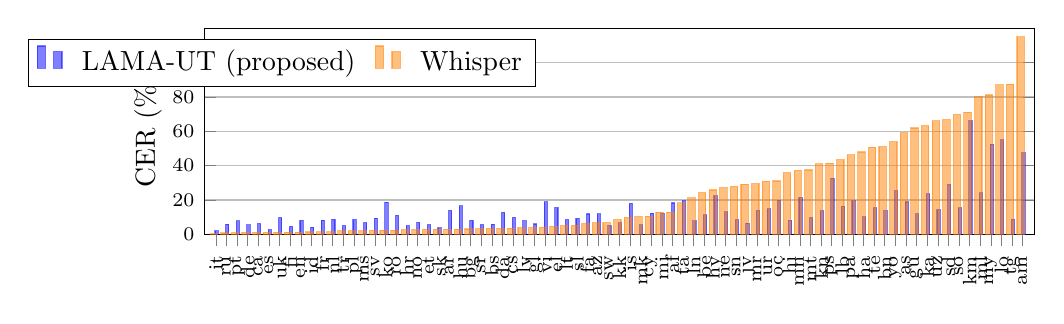
\begin{tikzpicture}
        \begin{axis}[
            width=\textwidth, 
            height=4.2cm, 
            ylabel={CER (\%)},
            ylabel style={yshift=-7pt},
            xtick={1,2,...,77}, 
            xticklabels={it, ru, pt, de, ca, es, uk, fi, en, id, fr, nl, tr, pl, ms, sv, ko, ro, hr, no, et, sk, ar, hu, bg, sr, bs, da, cs, lv, gl, vi, el, lt, sl, fa, az, sw, kk, is, mk, cy, mi, af, ta, ln, be, hy, ne, sn, jv, mr, ur, oc, hi, mn, mt, kn, ps, lb, pa, ha, te, bn, yo, as, gu, ka, uz, sd, so, km, ml, my, lo, tg, am
            },
            x tick label style={rotate=90, font=\scriptsize},
            xtick pos=bottom,
            grid=major, 
            xmajorgrids=false,
            legend style={at={(0.4,0.95)}, column sep=5pt},%, anchor=south east},
            % legend cell align={left},
            % legend style={at={(0.5, 1)},
            legend cell align={left},
            legend columns=2,
            ymin=0, ymax=120., 
            ytick={0, 20, 40, 60, 80, 100},
            y tick label style={font=\scriptsize},
            xmin=-0.1, xmax=78.1,
            ybar,
            ]
        
        \addplot+[style={blue, opacity=0.5, bar width=0.3, xshift=0.065cm}] 
            coordinates {(1, 2.0434) (2, 5.9955) (3, 7.8678) (4, 5.5343) (5, 6.3371) (6, 2.8268) (7, 9.7158) (8, 4.6651) (9, 8.1988) (10, 4.2642) (11, 8.2475) (12, 8.7417) (13, 5.1053) (14, 8.641) (15, 6.9177) (16, 9.4787) (17, 18.8081) (18, 11.0193) (19, 5.1653) (20, 6.9627) (21, 5.7385) (22, 3.802) (23, 13.936) (24, 16.6712) (25, 8.165) (26, 5.6728) (27, 5.934) (28, 12.8908) (29, 9.879) (30, 7.9353) (31, 6.0453) (32, 18.996) (33, 15.6008) (34, 8.6398) (35, 9.3782) (36, 11.8909) (37, 11.9132) (38, 5.297) (39, 6.7) (40, 18.1172) (41, 5.5156) (42, 12.3207) (43, 12.0296) (44, 18.294) (45, 19.578) (46, 7.8321) (47, 11.334) (48, 22.4033) (49, 13.1836) (50, 8.6191) (51, 6.5947) (52, 14.0207) (53, 14.906) (54, 19.8681) (55, 8.262) (56, 21.4495) (57, 9.8208) (58, 13.8512) (59, 32.7213) (60, 16.4643) (61, 19.5122) (62, 10.1785) (63, 15.4543) (64, 13.7857) (65, 25.5422) (66, 18.8821) (67, 11.9323) (68, 23.5731) (69, 14.4503) (70, 29.063) (71, 15.4388) (72, 66.2708) (73, 24.1487) (74, 52.5678) (75, 55.0304) (76, 8.8922) (77, 47.412)
            };
        \addplot+[style={orange, opacity=0.5, bar width=0.7, xshift=-0.108cm}] 
            coordinates {(1, 0.5042) (2, 0.8322) (3, 1.0532) (4, 1.125) (5, 1.1619) (6, 1.2367) (7, 1.262) (8, 1.3227) (9, 1.3455) (10, 1.4227) (11, 1.4741) (12, 1.5291) (13, 2.0229) (14, 2.0259) (15, 2.1292) (16, 2.2921) (17, 2.435) (18, 2.439) (19, 2.7453) (20, 2.7863) (21, 2.8731) (22, 2.95) (23, 2.9691) (24, 3.0123) (25, 3.1288) (26, 3.2842) (27, 3.5021) (28, 3.5785) (29, 3.6759) (30, 3.9959) (31, 4.0121) (32, 4.1578) (33, 4.7334) (34, 5.0884) (35, 5.2598) (36, 6.2866) (37, 6.8326) (38, 6.8898) (39, 8.5976) (40, 9.8542) (41, 10.3047) (42, 10.5821) (43, 12.9372) (44, 12.9688) (45, 18.3992) (46, 21.3185) (47, 24.3413) (48, 25.8559) (49, 27.2432) (50, 27.9583) (51, 29.2573) (52, 29.5538) (53, 30.9432) (54, 31.085) (55, 35.9342) (56, 37.2523) (57, 37.4938) (58, 41.0351) (59, 41.4955) (60, 43.4683) (61, 46.3415) (62, 47.9747) (63, 50.7616) (64, 51.0178) (65, 53.9499) (66, 59.2416) (67, 61.9198) (68, 63.2461) (69, 66.0443) (70, 66.866) (71, 69.925) (72, 71.1143) (73, 80.2781) (74, 81.1047) (75, 87.0318) (76, 87.4952) (77, 115.0166)};
        
        \legend{LAMA-UT (proposed)\qquad, Whisper}
        \end{axis}
    \end{tikzpicture}
    \caption{CER comparison between \shortname~and Whisper}
    \label{fig:histogram}
\end{figure*}

\section{Results}
Table~\ref{brief_comp_tab} shows that \shortname~effectively achieves multilingual ASR with a universal model.
This approach even operates in a zero-shot environment without requiring language-specific modules while utilizing only a minimal amount of training data.
In the subsequent results, we aim to validate the performance of each component within the pipeline.

\subsection{Universal Transcription Generator}
\subsubsection{Comparison to Baseline Model.}
We conducted a performance comparison between our universal transcription generator and the existing baseline, wav2vec2 phoneme~\cite{xu2021simpleeffectivezeroshotcrosslingual}. Our universal transcription generator focuses on generating character-level tokens and is measured using Character Error Rate (CER), while the baseline wav2vec2 phoneme is measured using Phoneme Error Rate (PER). However, since both metrics are fundamentally used for estimating phonetic symbols, this comparison can be considered meaningful.
Following the Table~\ref{orthography_comp_tab}, the results show that the proposed method demonstrated significantly better performance across a broader range of languages compared to existing approaches even not utilizing language-specific modules (e.g. n-gram LM).
Furthermore, our pipeline demonstrated relatively strong transcription capabilities for unseen languages that were not explicitly included in the training data.
In conclusion, transcribing diverse languages based on their pronunciation can produce a universal transcription which is highly effective.

\subsubsection{Orthography Unification Methods.} 
Among the two methods for standardizing orthographic features, Romanization proved to be more effective than IPA. 
Its ability to represent pronunciation across languages while reducing complexity makes it a superior choice for meaningful results.
Romanization balances phonetic accuracy with simplicity, providing better alignment with LLMs and ensuring efficient processing across multilingual ASR tasks.
 However, since these results are only constrained to the first phase of the pipeline, we have constructed the full end-to-end performance comparison between IPA-based and Romanization-based \shortname, and the results are shown in the appendix.

\subsection{Universal Converter Verification}
Despite the effectiveness of orthography unification, the success of the entire pipeline hinges on the proper functioning of the universal converter. Therefore, the most critical aspect to validate before experimentation was whether a frozen LLM could effectively serve as a universal converter.
To validate this objective, we passed ground truth Romanized transcriptions into the frozen universal converter and assessed its performance. This approach not only tests the converter's capability to accurately produce language-specific transcriptions but also serves to evaluate the upper bound performance of the universal converter within the proposed ASR pipeline.
In Table~\ref{upper_bound_tab}, results demonstrated that universal transcription based on pronunciation characteristics can yield significant performance improvements compared to previous works when the universal transcription generator operates ideally.
However, the upper bound performance for unseen languages showed a slight decrease compared to seen languages. 
This decrease is likely because the unseen languages we tested are typically extremely low-resource languages within the training data of the LLM.

\begin{table*}[]
\centering
\small
\begin{tabular}{c||c|cc|cc|cc|cc|cc}
\toprule
\multirow{4}{*}{Model} & \multirow{4}{*}{\begin{tabular}[c]{@{}c@{}}Repetition \\ \enspace Rate (\%) $\downarrow$  \end{tabular}}  & \multicolumn{10}{c}{Prompting Strategy}                                          \\ %cline{3-12}%\cmidrule{3-12}
                        & & \multicolumn{2}{c}{Zero-Shot} & \multicolumn{2}{c}{\begin{tabular}[c]{@{}c@{}}Few-Shot (5)\end{tabular}} & \multicolumn{2}{c}{Zero-Shot CoT} & \multicolumn{2}{c}{\begin{tabular}[c]{@{}c@{}}Few-Shot (5) +\\ Zero-Shot CoT\end{tabular}} & \multicolumn{2}{c}{\begin{tabular}[c]{@{}c@{}}Prompt\\ Chaining\end{tabular}} \\
                       &  & CER $\downarrow$           & WER $\downarrow$           & CER $\downarrow$                                  & WER $\downarrow$                                 & CER $\downarrow$                                 & WER $\downarrow$                                 & CER $\downarrow$                                       & WER $\downarrow$                                      & CER $\downarrow$                                  & WER $\downarrow$                                  \\ \midrule\midrule
 LLaMA-8B                      & 12        &  35.1             & 70.6              &   22.7                                   &                        49.6             &   37.2                                   &  77.4                                    &    22.1                                      &                                       49.8    &              35.9                        &                              70.8         \\
                        LLaMA-70B           & 1          &       24.3        &        53.8       &       17.4                               &        43.8                             &                       25.4               &     54.6                                 &          16.8                                  &                      43.7                     &      26.7                                 &         55.2                              \\
                        \textbf{GPT-4o-mini}      & \textbf{0.2}               &        \textbf{16.6}       &     \textbf{39.3}          &           \textbf{15.3}                           &                      \textbf{37.2}               &                           18.2           &         41.0                           &                     15.7            &          37.9   &      16.9          &               38.7                   \\ \bottomrule     
\end{tabular}%
\caption{Effects of prompting strategy and model type on the universal converter. The repetition rate indicates the proportion of samples with format errors (e.g., no section enclosed in three backticks until the maximum token limit) due to word repetition.}
\label{tab_ablation}
\end{table*}
\begin{table}[]
\centering
\small
\begin{tabular}{l|cccc}
\toprule
Model       &      \begin{tabular}[c]{@{}c@{}}Data (h)\end{tabular} & \begin{tabular}[c]{@{}c@{}}\# Lang.\end{tabular} & \begin{tabular}[c]{@{}c@{}}Universal\end{tabular} & CER $\downarrow$  \\ \midrule
ASR-2K & 2k & 8 & O                                             & 65.5 \\
% \textbf{\shortname} (IPA)         & \textbf{0.6k} & \textbf{102} & \textbf{O}                                                           & \textbf{40.4} \\
\textbf{\shortname} (Roman)        & \textbf{0.6k} & \textbf{102} & \textbf{O}                                                           & \textbf{34.7} \\
\midrule
MMS-ZS & 40k & 1078 & X                                              & 29.2 \\
+ n-gram LM & 40k & 1078 & X                                           & 25.2 \\
 \bottomrule
\end{tabular}%
\caption{
Comparison with previous zero-shot approaches. 
We evaluated transcription quality on 25 unseen languages from the CommonVoice 17.0 dataset. \textit{\# Lang.} denotes the number of languages leveraged in training.}
\label{unseen_comp_tab}
\end{table}
\subsection{Overall Pipeline}
\subsubsection{Seen Languages.}
We leveraged two baseline models for comparison: Whisper and MMS.
In Table~\ref{baseline_comparison_tab}, results demonstrate that the proposed method achieved a relative reduction of 60\% in CER and 30\% in WER compared to Whisper.
Moreover,~\shortname~matches the performance of MMS despite the absence of language-specific adapters, heads, and n-gram LMs.
Notably, the performance improvements were most pronounced for low-resource languages. 
While Whisper exhibited increased error rates for these languages due to limited training data, our method showed substantial performance enhancements with minimal data resources. 
Despite the slight performance degradation in high-resource languages, the improvement observed in low-resource languages is remarkably meaningful.
The full comparison results are presented in Fig~\ref{fig:histogram}.
It is noteworthy that these results were achieved with considerably smaller training data compared to Whisper and MMS.

\subsubsection{Unseen Languages.}
Our main focus was developing a generalized pipeline that demonstrates strong performance with unseen languages.
To validate this objective, we utilized two zero-shot ASR models as baselines: ASR-2K and Zero-Shot MMS (MMS-ZS).
In Table~\ref{unseen_comp_tab}, our method demonstrated a reduction in CER by half while using significantly less training data compared to ASR-2K.
Furthermore, it is noteworthy that our proposed pipeline performs remarkably well even without language-specific modules, demonstrating comparable performance to MMS-ZS which leverages language-specific lexicon and n-gram LM.

\subsection{Ablation Study}
\subsubsection{Prompting Strategy.}
In Table~\ref{tab_ablation}, few-shot prompting showed the highest performance across all models and prompting strategies.
Interestingly, even with zero-shot prompting, the proposed pipeline consistently outperforms Whisper on average in CER and WER, where Whisper records 23.9\% and 42.9\% respectively, as shown in Table~\ref{baseline_comparison_tab}.
On the other hand, the use of sequential reasoning failed to achieve the anticipated improvements. 
Specifically, we observed considerable error propagation when utilizing zero-shot CoT prompts and prompt chaining techniques.
Minor inaccuracies in the Romanization phase were amplified as they were processed by the LLM, leading to transcriptions that deviated in meaning from the intended output.

\subsubsection{Model Size and Training Data.}
From the perspective of model size, using a relatively smaller LLM like LLaMA-8B frequently resulted in issues such as word repetition, which complicated the transcription sorting process. 
Additionally, this model faced challenges with language misprediction, often generating transcriptions in languages other than the intended target language.
This issue was particularly noticeable with low-resource languages such as Arabic. 
With the LLaMA-70B model, while word repetition was less pronounced compared to the LLaMA-8B model, the issue of language misprediction persisted, albeit at a reduced frequency. 
Among the LLMs tested, GPT-4o-mini demonstrated the best performance overall. It outperformed the other models across all prompting strategies, achieving an impressive average CER of 15\% across 102 languages.
